\subsection{Hash Functions}
Hash functions are used for integrity protection. 
\begin{itemize}
    \item Blackbox function that takes an input and produces a fixed-size output
    \item Hash functions are deterministic, i.e., same input always produces the same output
    \item No matter how much data you give it, alwahys produces a fixed-size output
    \item Hash functions are fast to compute
    \item You can't reverse or predict the hash (one-way functions)
    \item Hash functions are collision resistant (only for SHA-256, not for MD5)
\end{itemize}

Asymmetric digital signature: sign hash of the document
MAC: Message Authentication Code, combine hash of message with secret key to obtain a MAC
Key generation

\subsubsection{Preimage Resistance}
Hash functions receive an arbitrary length bit string. They output a fixed length string called the hash value, digest, or hashcode. Cryptographic hash functions are one-way: easy to compute $y$ given $x$ but infeasible to find $x$ given $y: H: \{0,1\}^* \rightarrow \{0,1\}^n$, with $H(x) = y$.

\begin{defn}
    A hash function $H$ is \textbf{preimage resistant} if given $y$, it is computationally infeasible to find $x$ such that $H(x) = y$.
    Given an output of $t$ bits, it should take $O(2^t)$ time to find a preimage ($x$ is preimage of $y$).
\end{defn}

\begin{defn}
    A hash function $H$ is \textbf{second preimage resistant} if given $m$, it is computationally infeasible to find $m'$ such that $H(m) = H(m')$.
\end{defn}

\begin{figure}[h!]
    \centering
    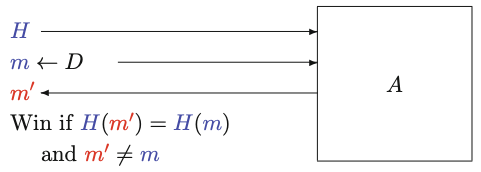
\includegraphics[width=0.35\textwidth]{img/2ndpreimage.png}
    \caption{Security game for second preimage resistance}
\end{figure}

This security game can be won by the adversary, because the domain of the message space (arbitrary length) is huge compared to the domain of the output. The output is fixed size, let's say 128. Then the domain is ``only'' $2^128$. There will be a number of collisions. 

\subsubsection{Collision Resistance}
Assume now that the domain is much larger than the co-domain. Given $H$, it should be infeasible to compute $m$ and $m'$ such that $H(m) = H(m')$.

\begin{defn}
    A hash function $H$ is \textbf{collision resistant} if it is computationally infeasible to find $m$ and $m'$ such that $H(m) = H(m')$.
    Given an output of $t$ bits, it should take $O(2^{t/2})$ time to find a collision.
\end{defn}

\begin{figure}[h!]
    \centering
    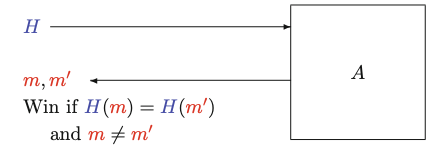
\includegraphics[width=0.35\textwidth]{img/col_resistance.png}
    \caption{Security game for collision resistance of a function}
\end{figure}

This security game can also be won by the adversary! There are several collusions: pigeonhole principle. We solved the same problem in PRFs by using a keyed version of the functions. However, we need unkeyed hash functions! This is because we need to be able to verify the integrity of the data without having the key (public use, no secret). Keyed hash functions are for security and authentication.

\begin{defn}
A function H is said to be collision resistant (by human
ignorance) or HI-CR secure if it is believed to be infeasible to write
down a collision for the function, i.e. two elements in the domain
mapping to the same element in the codomain.
\end{defn}

The probability to have a collision is $\sqrt{2^{t+1}}$ (Birthday paradox). \\

In summary, a cryptographic hash function:
\begin{enumerate}
    \item Preimage Resistant: It should be hard to find a message with
    a given hash value
    \item Second Preimage Resistant: Given one message it should be
    hard to find another message with the same hash value
    \item Collision Resistant: It should be hard to find two messages
    with the same hash value
\end{enumerate}

(1) is weaker than (2) and (3), (2) is weaker than (3). Some more terminology:

\begin{itemize}
    \item one-way = preimage + second preimage resistant
    \item weak collision resistant = second preimage resistant
    \item strong collision resistant = collision resistant
    \item OWHF = one-way hash function = preimage and second preimage resistant
    \item CRHF = collision resistant hash function = collision resistant and second preimage resistant
\end{itemize}

\subsection{Padding}
Even though the input size can be arbitrary, many hash algorithms process data in fixed-size blocks (e.g., 512-bit blocks for SHA-256). If the input data is not a multiple of the block size, padding is added to make the data fit perfectly into blocks.
Padding also helps to include the original message length in the hash calculation, which is crucial for preventing certain types of attacks (like length-extension attacks). \\

When you divide a message into smaller blocks, how can you pad it? Given an $l$ bit message $m$, and block size $b$, we want to have $m$ of length $kb$:
\[ m || \text{pad}_i(|m|, b) \]

In theory, padding can be applied at the beginning or the end. In practice, all algorithms pat at the end. \\

\subsubsection{Padding Methods}
We define 5 of them:

\begin{itemize}
    \item \textbf{Method 0:} $v = b - |m| \mod b$ and padding is $v$ zeros: $m||0^*$. In other words, the message is padded with zeros until it is a multiple of the block size
    \item \textbf{Method 1:} $v = b - (|m|+1) \mod b$ and padding is: $m||10^*$.
    \item \textbf{Method 2:} $v = b - (|m|+65) \mod b$ and padding is: $m||10^*||L$, where $L$ is a 64-bit integer encoding of $|m|$
    \item \textbf{Method 3:} $v = b - (|m|+64) \mod b$ and padding is: $m||0^*||L$
    \item \textbf{Method 4:} $v = b - (|m|+2) \mod b$ and padding is: $m||10^*1$
\end{itemize}

Any can be used, apart from method 0, but will effect security. Method 1 is also not good. \\

For SHA-256: The input message is padded by appending a 1 bit, followed by enough 0 bits, so that the total length is 64 bits short of a multiple of 512. Then, the original message length (in bits) is added as a 64-bit value at the end of the padded message.

\subsection{Merkle-Damg\aa rd Construction}
\begin{defn}
    A \textbf{compression function} is a hash function that takes an input and produces a fixed-size output. It is applied iteratively to compress larger inputs into a smaller output. After all blocks are processed, the final state becomes the output of the hash function.
\end{defn}

The MD construction is a method for building cryptographic hash functions. The construction breaks down the process of hashing into a series of steps where the input data is processed in fixed-size blocks. The key idea is to iteratively compress these blocks using a compression function.

\begin{figure}[h!]
    \centering
    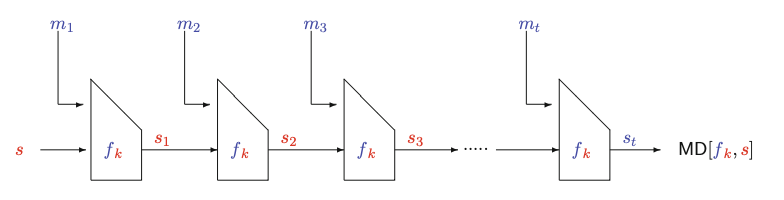
\includegraphics[width=0.5\textwidth]{img/MDconstruction.png}
    \caption{The Merkle-Damg\aa rd Construction MD$[f_k, s]$, where $s$ is the internal state}
\end{figure}

If the compression function is secure, then the hash function is secure too. 

\subsubsection{MD Algorithm}
\begin{itemize}
    \item Divide the innput message into fixed-size blocks. Apply padding if the message length is not a multiple of the block size.
    \item The process begins with an initial value (IV), a predefined set of constants.
    \item Iteratively apply the compression function $f_k$ to each block, taking the current state and block of data as input. The output of the compression function becomes the new state passed to the next iteration.
    \item After all blocks are processed, the final state becomes the final hash output.
\end{itemize}

\begin{figure}[h!]
    \centering
    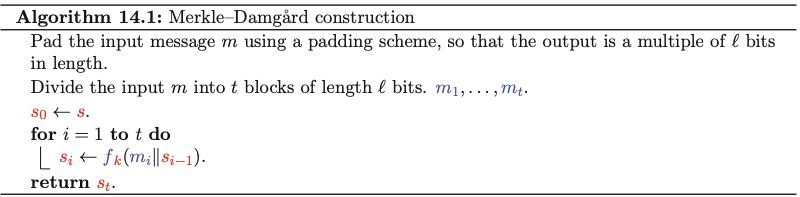
\includegraphics[width=0.6\textwidth]{img/MDalgorithm.png}
\end{figure}

\subsubsection{Benefits of MD Construction}
\begin{itemize}
\item Design makes streaming possible
\item Hash function analysis becomes compression function analysis
\item Analysis is easier because the domain of CF is finite
\end{itemize}

\subsubsection{Properties of MD Construction}
Collision resistance of the hash function depends on the padding method. Imagine there are two messages $m=0b0$ and $m'=0b00$. 
Using method 0, both of them will be mapped to $0b0000 \rightarrow$ collision.
This means that the original message can be $0b0, 0b00, 0b000, 0b0000$. All of them will be mapped to the same value.
Thus, MD-based hash function should \emph{not} use padding method 0. Use method 2 instead.

\subsubsection{Security properties under different scenarios}
\begin{enumerate}
    \item \textbf{\( s \) is fixed to an IV, \( f_k \) is also fixed:}
    \begin{itemize}
        \item \( s \) is initialized to a fixed Initial Value (IV), and \( f_k \), the compression function, is also fixed.
        \item If \( f \) is \textbf{HI-CR secure} (Highly Iterated Collision-Resistant), then the hash function \( H(m) \), constructed using the MD construction, is also collision-resistant.
        \item \textbf{Practical Use:} This describes the standard cryptographic hash functions where the IV and compression function are predefined.
    \end{itemize}
    
    \item \textbf{\( s_0 \) is a key, \( f_k \) is a fixed function:}
    \begin{itemize}
        \item Here, \( s_0 \) is treated as a \textbf{key} (instead of a fixed IV), while \( f_k \), the compression function, remains fixed.
        \item If \( f \) is \textbf{HI-CR secure}, the keyed hash function \( H_s(m) \) (where \( s_0 \) is the key) is also collision-resistant.
        \item \textbf{Practical Use:} This construction aligns with setups like HMAC, where a secret key is combined with the message for added security.
    \end{itemize}
    
    \item \textbf{\( f_k \) is from a PRF family, \( s \) is fixed:}
    \begin{itemize}
        \item In this case, \( f_k \) comes from a \textbf{PRF family}, and \( s \) (the initial value) is fixed.
        \item If \( f \) is \textbf{CR secure} (Collision-Resistant), then \( H_k(m) \), constructed using the MD process, is also collision-resistant. However, this setup has limited practical implications.
        \item \textbf{Practical Use:} This is more of a theoretical observation, as using a PRF family for \( f_k \) doesn’t add significant value for hashing in practice.
    \end{itemize}
\end{enumerate}

\subsection{MD-4}
MD-family is a series of hash functions: MD construction with a (fixed) \emph{unkeyed} compression function $f$. 
In MD-4 (128-bit output), the function f has 3 rounds of 16 steps each.

\begin{figure}[h!]
    \centering
    \begin{subfigure}{0.4\textwidth}
        \centering
        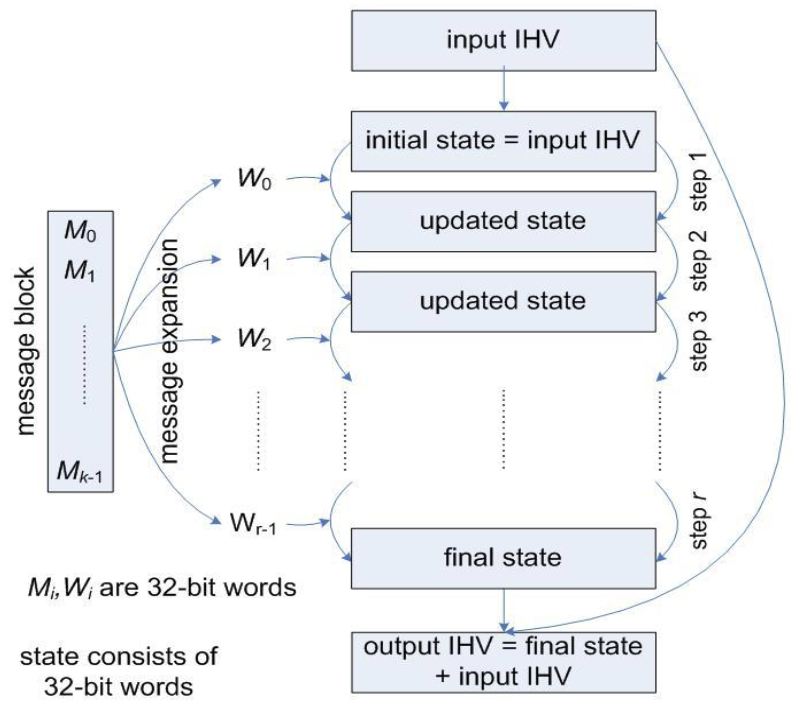
\includegraphics[width=0.9\textwidth]{img/md4.png}
        \caption{MD-4 compression function}
    \end{subfigure}
    \hfill
    \begin{subfigure}{0.4\textwidth}
        \centering
        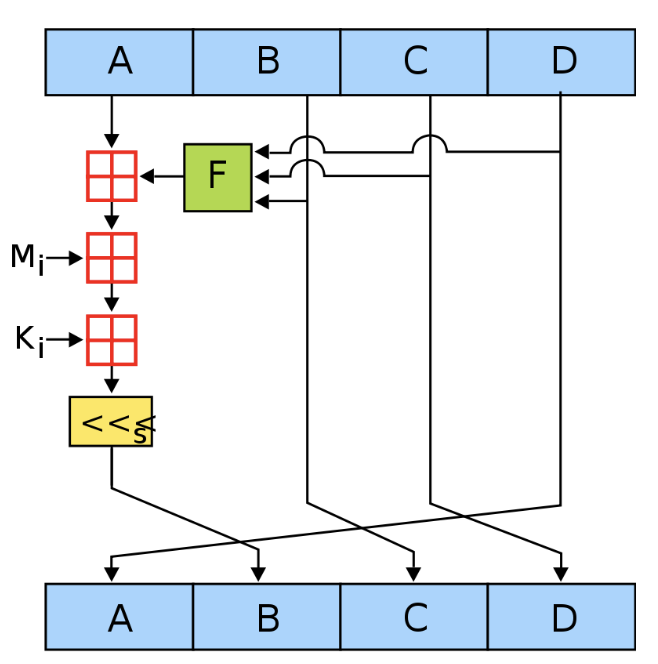
\includegraphics[width=0.9\textwidth]{img/md4steps.png}
        \caption{Steps in MD-4}
    \end{subfigure}
    \caption{MD-4 Compression Function and Steps}
\end{figure}

MD-4 is not secure, and should not be used in cryptographic applications. Vulnerable to collision attacks, these days collisions can be found in seconds. Also weak against (second) preimage attacks. \\
Risks associated with MD-4:
\begin{itemize}
    \item Digital signatures: If MD4 is used in signatures, an attacker can create fake documents with valid signatures by exploiting collisions.
    \item Data integrity: MD4 cannot reliably ensure data integrity, as attackers can manipulate data without detection.
\end{itemize}

MD4 has been superseded by much stronger algorithms, such as:
\begin{itemize}
    \item MD5 (although MD5 is also now considered insecure)
    \item SHA-1 (also insecure, with known collision attacks since 2017)
    \item SHA-2 and SHA-3 (currently secure)
\end{itemize}

\subsection{Birthday Paradox}
The \textbf{birthday paradox} refers to the counterintuitive probability that in a group of just 23 people, there is about a 50\% chance that two of them share the same birthday.

\subsubsection{Why does this happen?}
\begin{itemize}
    \item Instead of calculating the chance of one specific match, we consider \textbf{any pair} of people matching, which grows quickly as the group size increases.
    \item The total number of pairs increases exponentially with the number of people:
    \[
    \binom{n}{2} = \frac{n(n-1)}{2}.
    \]
\end{itemize}

Given a set of $t \geq 10$ elements, take a sample of size $k$ (drawn with repetition) in order to get a probability $/geq \frac{1}{2}$ on a collision. $k$ has to be larger than $1.2\sqrt{t}$.
Consequence: if $F: A \rightarrow B$ is a random function, and $\#A >> \#B$, then one can expect a collision after $\sqrt{\#B}$ random function calls. 

\subsubsection{In Cryptography}
\begin{itemize}
    \item The birthday paradox is used to explain the likelihood of \textbf{collisions} in hash functions.
    \item For a hash function with \( n \)-bit outputs:
    \begin{itemize}
        \item A collision is expected after approximately \( \sqrt{2^n} \) hashes, i.e., \( \approx 2^{n/2} \), due to the birthday paradox.
    \end{itemize}
    \item This highlights why hash functions need \textbf{large output sizes} (e.g., 256 bits) to prevent collisions.
\end{itemize}

\subsubsection{Random vs. Meaningful Birthdaying}
\begin{defn}
    \textbf{Random Birthdaying:} searching for any two inputs that produce the same output in a hash function, without any specific requirements on the inputs. Do an exhaustive search on $1/2n$ bits. The messages will be random and not meaningful. 
    Demonstrates the general weakness of a hash function if collisions can be found easily.
\end{defn}

\begin{defn}
    \textbf{Meaningful Birthdaying:}  finding a collision where at least one of the inputs has specific, meaningful content. 
    Start with two meaningful messages $m_1, m_2$ for which you want to find a collision.
    Identify $1/2n$ independent positions where the messages can be changed at bit-level without changing the meaning, e.g. tab—space, space—newline, etc. Do random search on those positions.
\end{defn}

\textbf{Note:} these are brute-force attacks.
\Comment{add an example here?}

\subsubsection{Implementing Birthdaying}
\begin{itemize}
    \item \textbf{Naïve}
    \begin{itemize}
        \item Store \( 2^{n/2} \) possible messages for \( m_1 \) and \( 2^{n/2} \) possible messages for \( m_2 \) and check all \( 2 \) pairs.
    \end{itemize}
    
    \item \textbf{Less naïve}
    \begin{itemize}
        \item Store \( 2^{n/2} \) possible messages for \( m_1 \), and for each possible \( m_2 \), check whether its hash is in the list.
    \end{itemize}
    
    \item \textbf{Smart:} Pollard-\(\rho\) with Floyd’s cycle-finding algorithm
    \begin{itemize}
        \item Computational complexity still \( O(2^{n/2}) \) – but only constant small storage required.
    \end{itemize}
\end{itemize}

\subsection{MAC and HMAC}
HMAC (Hash-based Message Authentication Code) is a cryptographic algorithm used to ensure both the integrity and authenticity of a message. 
It combines a cryptographic hash function (like SHA-256) with a secret key.

\subsubsection{Insecurity of Naïve Keyed Hash Construction}
A naïve attempt to create a keyed hash using an \emph{unkeyed} hash function is:

\[ t=H(k|| m || \text{pad}_i(|k|+|m|,b)) \]

where
\begin{itemize}
    \item $H$: unkeyed hash function
    \item $k$: secret key
    \item $m$: message
    \item pad$_i$: padding to ensure the input meets the block size of 
    \item This approach involves concatenating the key $k$, message $m$ and some padding before hashing.
\end{itemize}

The digest $t$ is then computed as:

\[ t=MD[f, s](k|| m || \text{pad}_i(|l|+|m|,l)) \]

where $MD[f, s]$ is the MD-hash function, and $l$ is the intermediate state. \\

The adversary can exploit this construction. If she can query $t$, she can then construct valid keyed hashes by appending additional data $m'$ to the message $m$.
This is called a \textbf{length extension attack}. Without knowing the secret key $k$, the attacker can extend the hash to new messages and generate valid keyed hashes. \\

A valid keyed hash for the new message can be computed as:

\[ m || pad_i(|l|+|m|,l) || m' \]

This construction allows an attacker to manipulate and extend the authenticated data.

\Comment{remove first block (key k), append corrupted message m'??}

\subsubsection{Secure Keyed Hash Construction}
We use nested MAC to construct a secure keyed hash function. The construction is as follows:

\[ \text{NMAC}_{k_1, k_2}(m) = F_{k_1} (F_{k_2}(m)) \]
\[ F_{k_1} = f((x || \text{pad}_2(l + |x|, l)) || k_1) = MD[f, k_1]^*(x)\]
\[ G_{k_2} = MD[f, k_2]^*(m) \]

But, we want one hash function with one key, so we construct HMAC as follows:

\[ \text{HMAC}_k(m) = H\left( (k \oplus \text{opad}) || H\left( (k \oplus \text{ipad}) || m \right) \right) \]
\[ = MD[f , IV ] ((k \oplus \text{opad}) ‖MD[f , IV ] ((k \oplus \text{ipad})) ||m )\]

or simplified:

\[ \text{Inner hash} = H(\text{ipad} || M) \]
\[ \text{HMAC} = H(\text{opad} || \text{Inner hash}) \]

\newpage

Steps in the process:
\begin{enumerate}
  \item \textbf{Key Preparation}:
  \begin{itemize}
    \item If the key is longer than the block size of the hash function, it is hashed first to reduce its size.
    \item If the key is shorter than the block size, it is padded with zeros to match the block size.
  \end{itemize}
  
  \item \textbf{Inner Hash Calculation}:
  \begin{itemize}
    \item XOR the key with a padding called the \textit{inner pad} (ipad).
    \item Concatenate the result with the original message.
    \item Hash the resulting data using the chosen hash function.
  \end{itemize}
  
  \item \textbf{Outer Hash Calculation}:
  \begin{itemize}
    \item XOR the key again, but this time with a different padding called the \textit{outer pad} (opad).
    \item Concatenate the result of the inner hash calculation with the outer padded key.
    \item Hash the resulting data.
  \end{itemize}
  
  \item \textbf{Output}: The final hash value after the second hash computation is the HMAC, which serves as the authentication code.
\end{enumerate}

\subsubsection{Security of HMAC}
The security of HMAC depends on the strength of the underlying hash function and the secrecy of the key. HMAC is resistant to various attacks, such as:
\begin{itemize}
  \item Brute-force attacks.
  \item Collision attacks.
  \item Length-extension attacks (common in some hash functions).
\end{itemize}

Suppose a client wants to send a message to a server, and both share a secret key:
\begin{enumerate}
  \item The client computes the HMAC of the message using the shared key.
  \item The client sends both the message and the HMAC to the server.
  \item The server computes the HMAC of the received message with the same key.
  \item If the computed HMAC matches the received HMAC, the server knows the message is authentic and unchanged.
\end{enumerate}

\subsection{Sponge Functions}
Sponge functions are a modern technique to create hash functions, MACs, key derivation functions, and more. They are based on the sponge construction, which is a generalization of the Merkle-Damg\aa rd construction. \\

It operates by absorbing input data and squeezing out output. The input and output can be of arbitrary length.
A sponge function works on an internal state, which is divided into two parts:
\begin{itemize}
  \item Capacity (c): The part that controls security.
  \item Rate (r): The part used for absorbing input and squeezing output.
\end{itemize}

\begin{figure}[h!]
    \centering
    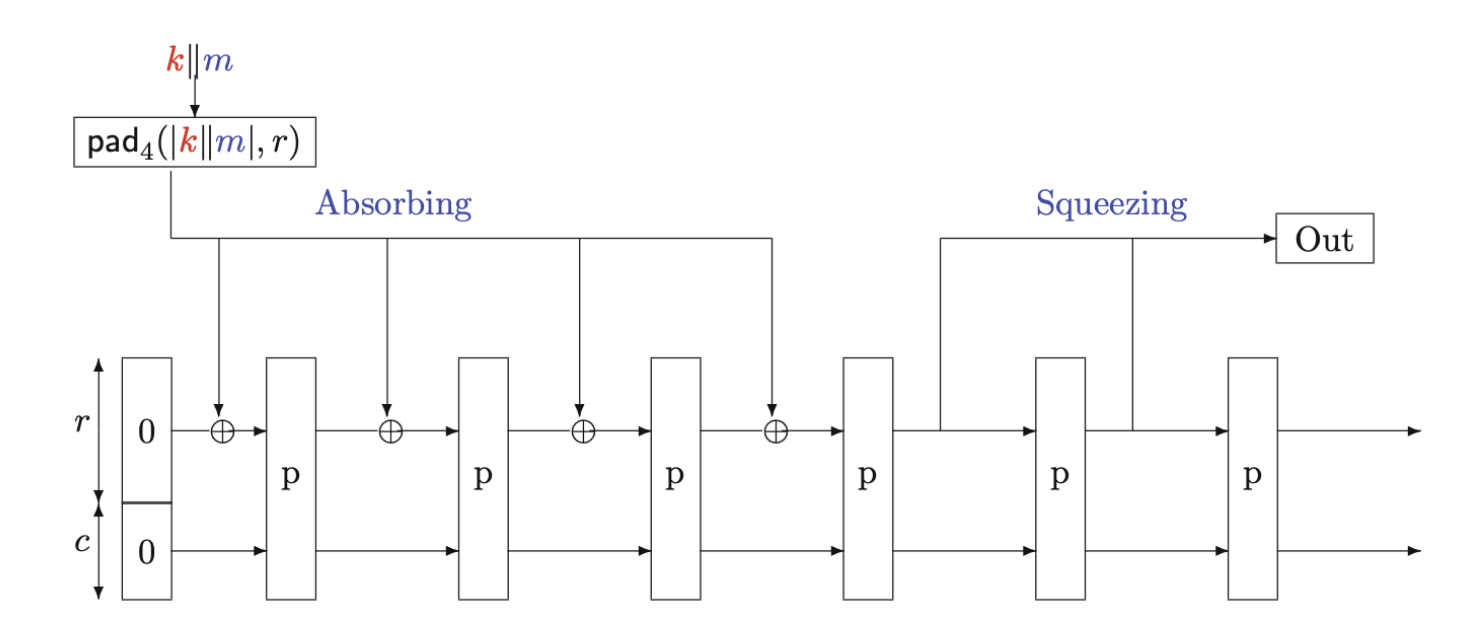
\includegraphics[width=0.7\textwidth]{img/sponge.png}
    \caption{Sponge construction $\text{SP}[p]$}
\end{figure}

Operations:
\begin{enumerate}
    \item \textbf{Absorbing Phase}: The input is divided into blocks and absorbed into the internal state by XORing with the rate portion, followed by a transformation (permutation) of the state:
    \[
    S = P(S \oplus M_i)
    \]
    where \( S \) is the state, \( M_i \) is the input block, and \( P \) is the permutation function.
    
    \item  \textbf{Squeezing Phase}: After all input is absorbed, the output is extracted from the rate portion of the state. Additional squeezing rounds can be performed if more output is needed:
    \[
    O = S_{\text{rate}} \quad \text{(extract the rate portion)}
    \]
\end{enumerate}

The security of a sponge function is based on the size of the capacity. Larger capacities make the function more resistant to collission and preimage attacks. \\

\textbf{Example: SHA-3 (Keccak)}
SHA-3, based on the Keccak sponge construction, has an internal state of 1600 bits, divided into 1024 bits for the rate and 576 bits for the capacity. The absorbing phase processes input in blocks of 1024 bits, and output is squeezed from the rate portion.
